% Created by tikzDevice version 0.12 on 2019-07-24 15:43:39
% !TEX encoding = UTF-8 Unicode
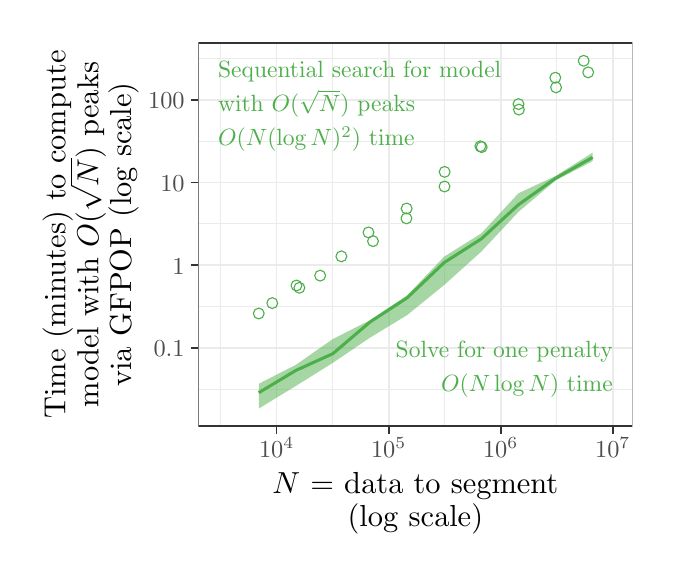
\begin{tikzpicture}[x=1pt,y=1pt]
\definecolor{fillColor}{RGB}{255,255,255}
\path[use as bounding box,fill=fillColor,fill opacity=0.00] (0,0) rectangle (224.04,187.90);
\begin{scope}
\path[clip] (  0.00,  0.00) rectangle (224.04,187.90);
\definecolor{drawColor}{RGB}{255,255,255}
\definecolor{fillColor}{RGB}{255,255,255}

\path[draw=drawColor,line width= 0.6pt,line join=round,line cap=round,fill=fillColor] (  0.00,  0.00) rectangle (224.04,187.90);
\end{scope}
\begin{scope}
\path[clip] ( 61.67, 43.96) rectangle (218.54,182.40);
\definecolor{fillColor}{RGB}{255,255,255}

\path[fill=fillColor] ( 61.67, 43.96) rectangle (218.54,182.40);
\definecolor{drawColor}{gray}{0.92}

\path[draw=drawColor,line width= 0.3pt,line join=round] ( 61.67, 57.25) --
	(218.54, 57.25);

\path[draw=drawColor,line width= 0.3pt,line join=round] ( 61.67, 87.14) --
	(218.54, 87.14);

\path[draw=drawColor,line width= 0.3pt,line join=round] ( 61.67,117.02) --
	(218.54,117.02);

\path[draw=drawColor,line width= 0.3pt,line join=round] ( 61.67,146.91) --
	(218.54,146.91);

\path[draw=drawColor,line width= 0.3pt,line join=round] ( 61.67,176.79) --
	(218.54,176.79);

\path[draw=drawColor,line width= 0.3pt,line join=round] ( 69.73, 43.96) --
	( 69.73,182.40);

\path[draw=drawColor,line width= 0.3pt,line join=round] (110.21, 43.96) --
	(110.21,182.40);

\path[draw=drawColor,line width= 0.3pt,line join=round] (150.69, 43.96) --
	(150.69,182.40);

\path[draw=drawColor,line width= 0.3pt,line join=round] (191.17, 43.96) --
	(191.17,182.40);

\path[draw=drawColor,line width= 0.6pt,line join=round] ( 61.67, 72.19) --
	(218.54, 72.19);

\path[draw=drawColor,line width= 0.6pt,line join=round] ( 61.67,102.08) --
	(218.54,102.08);

\path[draw=drawColor,line width= 0.6pt,line join=round] ( 61.67,131.96) --
	(218.54,131.96);

\path[draw=drawColor,line width= 0.6pt,line join=round] ( 61.67,161.85) --
	(218.54,161.85);

\path[draw=drawColor,line width= 0.6pt,line join=round] ( 89.97, 43.96) --
	( 89.97,182.40);

\path[draw=drawColor,line width= 0.6pt,line join=round] (130.45, 43.96) --
	(130.45,182.40);

\path[draw=drawColor,line width= 0.6pt,line join=round] (170.93, 43.96) --
	(170.93,182.40);

\path[draw=drawColor,line width= 0.6pt,line join=round] (211.41, 43.96) --
	(211.41,182.40);
\definecolor{drawColor}{RGB}{77,175,74}

\node[text=drawColor,anchor=base west,inner sep=0pt, outer sep=0pt, scale=  0.85] at ( 68.80,169.80) {Sequential search for model};

\node[text=drawColor,anchor=base west,inner sep=0pt, outer sep=0pt, scale=  0.85] at ( 68.80,157.51) {with $O(\sqrt N)$ peaks};

\node[text=drawColor,anchor=base west,inner sep=0pt, outer sep=0pt, scale=  0.85] at ( 68.80,145.22) {$O(N(\log N)^2)$ time};

\node[text=drawColor,anchor=base east,inner sep=0pt, outer sep=0pt, scale=  0.85] at (211.41, 68.86) {Solve for one penalty};

\node[text=drawColor,anchor=base east,inner sep=0pt, outer sep=0pt, scale=  0.85] at (211.41, 56.57) {$O(N \log N)$ time};
\definecolor{fillColor}{RGB}{77,175,74}

\path[fill=fillColor,fill opacity=0.50] ( 83.50, 59.22) --
	( 96.90, 66.06) --
	(110.31, 75.42) --
	(123.71, 82.18) --
	(137.12, 91.16) --
	(150.53,105.17) --
	(163.93,113.57) --
	(177.34,128.06) --
	(190.75,134.30) --
	(204.15,142.73) --
	(204.15,139.67) --
	(190.75,132.70) --
	(177.34,121.33) --
	(163.93,107.01) --
	(150.53, 94.94) --
	(137.12, 84.04) --
	(123.71, 75.90) --
	(110.31, 66.81) --
	( 96.90, 58.44) --
	( 83.50, 50.26) --
	cycle;

\path[draw=drawColor,line width= 1.1pt,line join=round] ( 83.50, 56.00) --
	( 96.90, 64.04) --
	(110.31, 70.12) --
	(123.71, 81.55) --
	(137.12, 90.28) --
	(150.53,103.04) --
	(163.93,111.59) --
	(177.34,123.93) --
	(190.75,133.48) --
	(204.15,141.02);

\path[draw=drawColor,line width= 0.4pt,line join=round,line cap=round] ( 83.50, 84.62) circle (  1.96);

\path[draw=drawColor,line width= 0.4pt,line join=round,line cap=round] ( 88.39, 88.37) circle (  1.96);

\path[draw=drawColor,line width= 0.4pt,line join=round,line cap=round] ( 97.12, 94.73) circle (  1.96);

\path[draw=drawColor,line width= 0.4pt,line join=round,line cap=round] ( 98.19, 93.90) circle (  1.96);

\path[draw=drawColor,line width= 0.4pt,line join=round,line cap=round] (105.69, 98.30) circle (  1.96);

\path[draw=drawColor,line width= 0.4pt,line join=round,line cap=round] (113.36,105.26) circle (  1.96);

\path[draw=drawColor,line width= 0.4pt,line join=round,line cap=round] (123.15,113.91) circle (  1.96);

\path[draw=drawColor,line width= 0.4pt,line join=round,line cap=round] (124.78,110.76) circle (  1.96);

\path[draw=drawColor,line width= 0.4pt,line join=round,line cap=round] (136.87,118.99) circle (  1.96);

\path[draw=drawColor,line width= 0.4pt,line join=round,line cap=round] (136.94,122.56) circle (  1.96);

\path[draw=drawColor,line width= 0.4pt,line join=round,line cap=round] (150.62,130.50) circle (  1.96);

\path[draw=drawColor,line width= 0.4pt,line join=round,line cap=round] (150.66,135.79) circle (  1.96);

\path[draw=drawColor,line width= 0.4pt,line join=round,line cap=round] (163.57,145.05) circle (  1.96);

\path[draw=drawColor,line width= 0.4pt,line join=round,line cap=round] (164.06,144.73) circle (  1.96);

\path[draw=drawColor,line width= 0.4pt,line join=round,line cap=round] (177.36,160.29) circle (  1.96);

\path[draw=drawColor,line width= 0.4pt,line join=round,line cap=round] (177.51,158.29) circle (  1.96);

\path[draw=drawColor,line width= 0.4pt,line join=round,line cap=round] (190.66,169.82) circle (  1.96);

\path[draw=drawColor,line width= 0.4pt,line join=round,line cap=round] (190.93,166.33) circle (  1.96);

\path[draw=drawColor,line width= 0.4pt,line join=round,line cap=round] (200.92,175.93) circle (  1.96);

\path[draw=drawColor,line width= 0.4pt,line join=round,line cap=round] (202.54,171.75) circle (  1.96);
\definecolor{drawColor}{gray}{0.20}

\path[draw=drawColor,line width= 0.6pt,line join=round,line cap=round] ( 61.67, 43.96) rectangle (218.54,182.40);
\end{scope}
\begin{scope}
\path[clip] (  0.00,  0.00) rectangle (224.04,187.90);
\definecolor{drawColor}{gray}{0.30}

\node[text=drawColor,anchor=base east,inner sep=0pt, outer sep=0pt, scale=  0.88] at ( 56.72, 68.94) {0.1};

\node[text=drawColor,anchor=base east,inner sep=0pt, outer sep=0pt, scale=  0.88] at ( 56.72, 98.83) {1};

\node[text=drawColor,anchor=base east,inner sep=0pt, outer sep=0pt, scale=  0.88] at ( 56.72,128.71) {10};

\node[text=drawColor,anchor=base east,inner sep=0pt, outer sep=0pt, scale=  0.88] at ( 56.72,158.60) {100};
\end{scope}
\begin{scope}
\path[clip] (  0.00,  0.00) rectangle (224.04,187.90);
\definecolor{drawColor}{gray}{0.20}

\path[draw=drawColor,line width= 0.6pt,line join=round] ( 58.92, 72.19) --
	( 61.67, 72.19);

\path[draw=drawColor,line width= 0.6pt,line join=round] ( 58.92,102.08) --
	( 61.67,102.08);

\path[draw=drawColor,line width= 0.6pt,line join=round] ( 58.92,131.96) --
	( 61.67,131.96);

\path[draw=drawColor,line width= 0.6pt,line join=round] ( 58.92,161.85) --
	( 61.67,161.85);
\end{scope}
\begin{scope}
\path[clip] (  0.00,  0.00) rectangle (224.04,187.90);
\definecolor{drawColor}{gray}{0.20}

\path[draw=drawColor,line width= 0.6pt,line join=round] ( 89.97, 41.21) --
	( 89.97, 43.96);

\path[draw=drawColor,line width= 0.6pt,line join=round] (130.45, 41.21) --
	(130.45, 43.96);

\path[draw=drawColor,line width= 0.6pt,line join=round] (170.93, 41.21) --
	(170.93, 43.96);

\path[draw=drawColor,line width= 0.6pt,line join=round] (211.41, 41.21) --
	(211.41, 43.96);
\end{scope}
\begin{scope}
\path[clip] (  0.00,  0.00) rectangle (224.04,187.90);
\definecolor{drawColor}{gray}{0.30}

\node[text=drawColor,anchor=base,inner sep=0pt, outer sep=0pt, scale=  0.88] at ( 89.97, 32.51) {$10^4$};

\node[text=drawColor,anchor=base,inner sep=0pt, outer sep=0pt, scale=  0.88] at (130.45, 32.51) {$10^5$};

\node[text=drawColor,anchor=base,inner sep=0pt, outer sep=0pt, scale=  0.88] at (170.93, 32.51) {$10^6$};

\node[text=drawColor,anchor=base,inner sep=0pt, outer sep=0pt, scale=  0.88] at (211.41, 32.51) {$10^7$};
\end{scope}
\begin{scope}
\path[clip] (  0.00,  0.00) rectangle (224.04,187.90);
\definecolor{drawColor}{RGB}{0,0,0}

\node[text=drawColor,anchor=base,inner sep=0pt, outer sep=0pt, scale=  1.10] at (140.10, 19.50) {$N$ = data to segment};

\node[text=drawColor,anchor=base,inner sep=0pt, outer sep=0pt, scale=  1.10] at (140.10,  7.62) {(log scale)};
\end{scope}
\begin{scope}
\path[clip] (  0.00,  0.00) rectangle (224.04,187.90);
\definecolor{drawColor}{RGB}{0,0,0}

\node[text=drawColor,rotate= 90.00,anchor=base,inner sep=0pt, outer sep=0pt, scale=  1.10] at ( 13.63,113.18) {Time (minutes) to compute};

\node[text=drawColor,rotate= 90.00,anchor=base,inner sep=0pt, outer sep=0pt, scale=  1.10] at ( 25.51,113.18) {     model with $O(\sqrt N)$ peaks};

\node[text=drawColor,rotate= 90.00,anchor=base,inner sep=0pt, outer sep=0pt, scale=  1.10] at ( 37.39,113.18) {     via GFPOP (log scale)};
\end{scope}
\end{tikzpicture}
